%\documentclass[11pt,letterpaper,twocolumn]{article}

%%%%%%%%%%%%%%%%%%%%%%%%%%%
%%%% SIN TANTA TÉCNICA %%%%
%%%%%%%%%%%%%%%%%%%%%%%%%%%

\documentclass[12pt,letterpaper, twoside, openright,
headinclude,footinclude,BCOR5mm,
numbers=noenddot,cleardoublepage=empty,
tablecaptionabove]{article}

\usepackage[utf8]{inputenc}
\usepackage[spanish]{babel}
\usepackage{amsmath}
\usepackage{amsfonts}
\usepackage{amssymb}
\usepackage{graphicx}
\usepackage{titling}
\setlength{\droptitle}{-5em}   % This is your set screw

\pretitle{
  \begin{center}
    \LARGE
    
  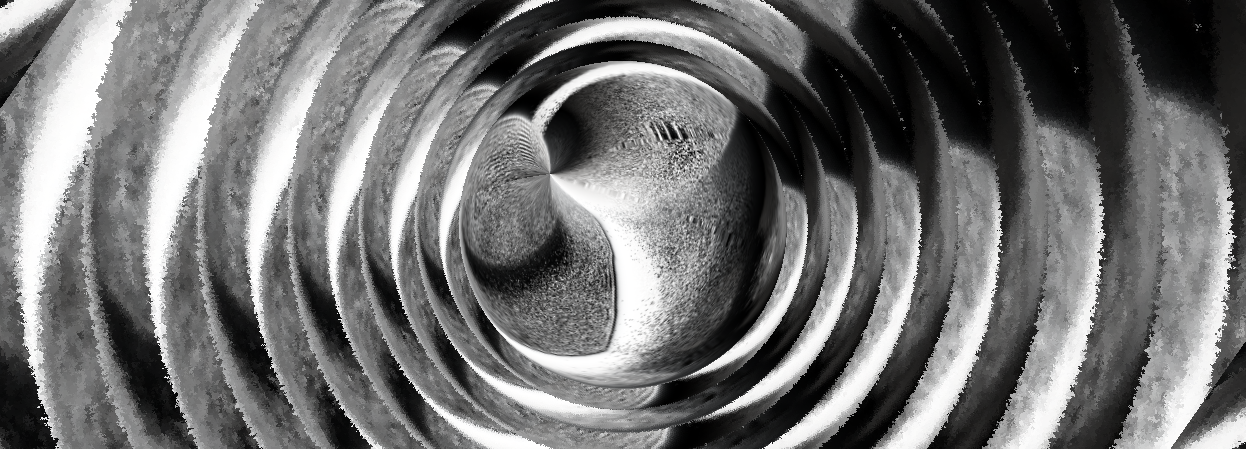
\includegraphics[width=0.5\textwidth]{../img/banner.png}\\[\bigskipamount]
}
\posttitle{\end{center}}


\usepackage{hyperref}
\usepackage[sort&compress]{natbib}
\usepackage{setspace}
%\usepackage{subfiles}
%\usepackage{graphicx}
\usepackage{subfig}
\usepackage[eulerchapternumbers,subfig,beramono,eulermath,pdfspacing]{classicthesis}
\usepackage{arsclassica}

\usepackage[letterpaper,
            bindingoffset=0in]{geometry}

\author{Emilio Ocelotl Reyes}
\title{Dos Anti Estudios} 
\begin{document}

\maketitle

\section*{Introducción}

Este proyecto describe un proceso de investigación-creación audiovisual en la web, inscrito en un ecosistema de escrituras de software semejantes. Parte de la investigación artística para relacionar práctica audiovisual con observaciones política y socialmente involucradas con ésta, de cara a una primera distinción: las escrituras que parten de la práctica artística, tanto para hacer obras como para ser obras en diferenciación con un contexto global que produce software como mercancía. 

El objetivo de esta reflexión consiste en describir la síntesis que resulta de los aspectos tecnológicos presentes en los lenguajes de programación y la escritura creativa y performática. De esta relación se desprende el espectro de prácticas en las cuales se inscribe la investigación, las piezas que la acompañan y algunas observaciones del ecosistema circundante. 

En este proyecto se retoman un conjunto de conceptos transversales, compartidos e históricamente conformados como: retroalimentación de múltiples instancias, el alejamiento y acercamiento en una escala de tiempo, la modularidad, el ensamblaje de proyectos pequeños y el error como corrupción pero también como un agente interlocutor. 

En el primer apartado se encuentran los antecedentes del proyecto, eventos y proyectos afines que han sido significativos. En el segundo y tercer apartado es posible encontrar las descripciones de THREE.studies y Anti, intercaladas con comentarios y reflexiones sobre proyectos y herramientas colindantes. En las conclusiones las reflexiones sobre las escrituras realizadas, los pendientes y el camino recorrido hasta el momento. 

\section*{Antecedentes}

% Las motivaciones generales de esta investigación refieren al interés por la reflexión vertida en investigación generada a partir de un proceso práctico y performático con sonido. Este trayecto ha involucrado imagen: actualmente, la realización de este bucle de investigación-creación es audiovisual.

% Este trabajo forma parte de una trilogía de investigación, junto con \emph{Objeto, Paisaje y Efecto} y \emph{Cuidado con la Brecha}. En este sentido, los estudios todavía-no-terminados-pero-abiertos forman parte de una trayectoria que problematiza la investigación sobre y con sonido e imagen. 

La práctica de la programación al vuelo o \emph{live coding} y la programación convencional con fines no-performáticos es una influencia notable para esta investigación. En \cite{villasenor} podemos encontrar referencias a la comunidad que practica la escritura al vuelo en México, que en algunos casos apunta hacia la escritura performática con salidas de audio y video pero que en otros casos se expresa en formatos, lugares y categorías de la música algorítmica\citep{jro2}. Este proceso de escritura de programas que unas veces es performático y otras veces persigue la fijación en el tiempo deriva en una propuesta que de fondo encuentra relaciones entre distintos tipos de escritura. Una característica distintiva del live coding es la comunidad que la promueve. Si bien esta investigación no se avoca específicamente al live coding, sí rescata las posibilidades de análisis que relaciona la socialización y la técnica con los sujetos que lo practican \citep{diProspero}. % Aquí podría poner el nucleo de una discusión que habla de la acción o lo performático en la palabrav

%Por aquí puede haber una referencia a la colaboración con Marianne, Luis, Celeste, Jessica, Hernani y el ensamble y Alejandro Brianza 

%% Imágenes o referencias a esto en la presentación. Me imagino algo tipo presentación anidada 

Las premisas del software y la cultura libre han sido fundamentales para el planteamiento del proyecto. La escritura de módulos y la puesta en marcha en un contexto comunitario de exploración creativa ha sido uno de los principales detonadores de las ideas que quedan presentes en las piezas y el resultado escrito de esta investigación. El software libre y de código abierto puede tener repercusiones en los resultados sonoros y visuales e incluso pueden ser herramientas pedagógicas para introducir conceptos que son comunes entre la práctica artística y la programación. También incide en las formas de organización social, económica y política \citep{jorgeDavid2021}. Algunos conceptos como la infraestructura, el cuidado, la distribución\footnote{``Can we code to care and code carefully?'' Taeyoon Choi. Consultado el \today en: \url{https://taeyoonchoi.com/soft-care/distributed-web-of-care/}} y el trabajo colaborativo en red \citep{hernaniRed} en contextos de escritura de código también son referencia para el proyecto. 

En 2018 el colectivo rggtrn impartió una serie de talleres que motivaron la reflexión en torno a la realización de interfaces textuales que pudieran responder a inquietudes específicas de usuarios que se acercan a la escritura de software \citep{bellacode}. El desarrollo de mini-lenguajes definidos localmente abonaron al proyecto de Luis Navarro y desembocaron en seis8s\footnote{https://github.com/luisnavarrodelangel/seis8s}. Sobre este punto, las consecuencias que giran en torno a Estuary como plataforma que promueve el aprendizaje de código al vuelo establece líneas de reflexión sobre pedagogía y diseño de interfaces textuales personalizadas.

%% Pie de nota sobre Estuary 

Por último, hay dos casos de piezas realizadas para la web que anteceden a esta investigación: Notas de Ausencia de Marianne Teixido\footnote{Consultado el \today en: \url{https://github.com/MarianneTeixido/notasdeausencia/}}. El segundo caso es Panorama\footnote{\url{https://github.com/piranhalab/panorama}}, un espacio inmersivo y libre para la realización de conciertos en la web.

%% Imagenes y referencias 

%% Aquí podría poner la referencia al proyecto de Aaron. Buscar el artículo en zenodo. 

\section*{Presencia y gesto}

\emph{THREE.studies} es una exploración para el navegador cuya premisa estética surge a partir de la implementación y mezcla de retroalimentaciones. Funciona como un sistema interactivo que renderea gráficos realizados con webGL por medio de Three.js y audio generado con SuperCollider.
 
% La elección de three.js como librería para gráficos. ¿Por qué? 

% No se si al inicio o al final pero en algún momento tengo ue hablar de los granos como consecuencia sonora y visual buscada 

El estudio estuvo pensado para el contexto de la copresencia digital. Inmerso en el contexto del trabajo con Panorama y sin la posibilidad de realizar ensayos presenciales, la pieza buscó soluciones al trabajo distanciado. Tomando en cuenta \emph{Cuidado con la brecha}, una investigación pasada sobre sistemas interactivos, el aspecto tecnológico de la pieza busco lidiar con la presencia distanciada del operador de la electrónica y  la interpretación instrumental. El eje articulador entre las investigaciones implicó un tránsito de sistemas interactivos instalados en computadoras de placa reducida a la escritura de programas para el navegador. El objetivo del trabajo en la web fue la portabilidad y el acceso que permite el despliegue de un sitio web sin instalaciones orientado a la interpretación audiovisual. La cero instalación como consecuencia y posibilidad está presente en plataformas como Estuary \citep{ogborn} e Hydra \citep{ojack}. % Hy

% Referencia a Cuidad con la brecha 

% Aclarar la descripción de abajo 

La primera versión de la pieza estuvo pensada como una partitura existente en el espacio tridimensional que pudiera dar cuenta de todos los procesos que sucedían durante la interpretación: la ejecución instrumental  enviaba señales de audio por medio de una conexión directa y que recibía por el mismo medio retroalimentación de la electrónica. La operación de la electrónica que para esta versión, fue ejecutada con código al vuelo y se proyectó como una suma de capas de ventanas transparentes en el escritorio. Los resultados visuales estaban previamente diseñados y respondían al audio de entrada. Esta superposición de capas de información permitió complejizar la entrada y salida de señales entre programas y plataformas. En este primer momento, surgió la pregunta: ¿Es posible desbordar este entramado hacia la investigación y hacia la reflexión? Como una pieza fija para el navegador, la pieza pudo participar en BEAST FEaST 2021\footnote{\url{http://www.beast.bham.ac.uk/beast-feast-2021/online-works/}}. Las pruebas fueron realizadas por medio de Sonobus y coordinadas por medio de una videollamada con Iracema de Andrade a cargo del cello eléctrico. 

%% Reactivar la liga

% Descripción técnica y comparación con algo o alusión a algunas tecnologías de las cuales supuestamente puedo ser especialista 

%% Cuál distanciamiento ? 

Para la segunda versión fue posible realizar algunas capturas presenciales que permitieron extender el continuo entre distanciamiento y presencia. El desplazamiento perseguido transitó del formato de video cuadrado a una captura tridimensional de superficies. El control de la electrónica y de los eventos que sucedían en el espacio 3d fue una mezcla de programación al vuelo con SuperCollider y la modificación de algunos parámetros gestuales en los visuales como la posición de la cámara o el recorrido de una muestra de audio con un control de videojuego. De estas propuestas emanaron reflexiones referentes a la ludificación de las interfaces y las piezas. 

% No se entiende bien la granulación 

La tercera versión parte de las premisas anteriores: retroalimentaciones basadas en la percepción auditiva y visual de la instrumentista. De manera similar a las versiones anteriores, es necesario transformar algunos parámetros del audio y la imagen con controladores externos, también ha sido necesario delimitar temporalmente algunos eventos de acuerdo a la narrativa de la pieza. Existe una relación entre la densidad de objetos en el dibujo y la densidad de granos en la muestra.  La densidad compartida define curvas que sugieren exploraciones generales del lado de la interpretación.

El resultado visual es una mezcla de técnicas que por un lado, manipula texturas generadas con Hydra y por el otro, las renderiza en objetos tridimensionales. Existe una segunda textura que se repite a sí misma. En el espacio digital, ambas texturas retroalimentadas coinciden, se intercalan e intercambian. Además de la densidad de granos, algunos parámetros presentes en los visuales que para esta ocasión fungen como partitura gráfica, son: resplandor de los objetos, difuminación, distorsión de texturas, cantidad, posición, rotación, escala y empalme de objetos, posición de la cámara y sensibilidad a la audioreactividad. En una búsqueda por la delimitación de la pieza, estos parámetros han sido traducidos para establecer las reglas de la interpretación / juego. THREE.studies aprovecha las tecnologías de los nuevos medios y participa en la tradición no nueva de utilizar notaciones gráficas y experimentos con tecnologías distintas a la escritura convencional de música, la indeterminación, los algoritmos y el papel activo que puede tener la interpretación en el proceso de co-creación musical y visual con tecnología \citep{magnussonSonic}. 

% Reactivar la liga 

%Retroalimentación 

%uturo 

%Ejercicios pequeños como lo del control

%Pendientes generales

%Reacción y retroalimentación perfomática con instrumentos y con código 

\section*{Ofuscación como motivo}

%% Esto primero está bueno, debería intercalar esto con ideas de la pieza 

La ofuscación puede definirse como el acto deliberado de encubrir el significado de una comunicación. Para el caso de la programación y apuntando ideas hacia los estudios del software, la presente investigación toma la noción de ofuscación para plantear la escritura de software que coincide, dialoga o se enfrenta alo que podríamos definir como la convención de la \emph{estética del código} basada en valoraciones de ``elegancia y belleza''\citep[p.~10]{EWD:EWD35} y aquellos programas que exploran ``otros principios estéticos'' como la aproximación lúdica de programas a partir de la ofuscación y la búsqueda de las diferentes dimensiones de sentido en la programación\citep[p.~198]{obfuscatedCode}

% Pregunta sobre si es subjetiva 

El código, su lectura y las funciones de los programas que ejecuta, son subjetivas y están determinadas por un sentido imputado que socialmente se acuerda de manera tácita y que puede ser visibilizado para confrontarlo en un sentido crítico, lúdico e incluso satírico.\footnote{Tal es el caso de Windows 93 del artista Jankenpopp. \url{https://www.windows93.net/} } En este punto encontramos conexiones con las posibilidades de la programación que resiste a la claridad y la elegancia, que resiste al lenguaje en el que está escrito\citep[p.~198]{obfuscatedCode}.

%% Esta raro 

La pregunta sobre sí el código fuente puede ``luchar'' en contra del marco de uso para el que fue escrito, en un amplio sentido tecnosocial, fue una de las motivaciones de Anti. Anti es un manual y una pieza para el navegador. Inicialmente estuvo pensada para explorar la ofuscación de audio y video. Adicionalmente, Anti fue un motivo para desplazar el proyecto hacia la escritura y la conformación de un ensayo interactivo para la web. El eje del proyecto giró en torno a la responsabilidad de los datos, al compromiso, al cuidado y a la realización de usuarios que desdibujan las fronteras de la pasividad política y económica teniendo como epicentro lo sensible.

\emph{Vocable Code}\footnote{\url{https://dobbeltdagger.net/VocableCode/}} de Winnie Soon en coescritura con Geoffrey Cox es un referente para la investigación en la medida que expresa práctica y reflexivamente la distinción entre \emph{software art} (software como obra de arte) y \emph{codework} (donde el código fuente y la escritura crítica operan conjuntamente.\footnote{Consultado el \today en: \url{https://dobbeltdagger.net/VocableCode/}}. Para el caso de Anti, la aproximación coincidió con la segunda definición: La escritura del programa y la escritura de reflexiones cortas que atravesaban temáticas tecnológicas, políticas y personales, sucedieron al mismo tiempo. Estas reflexiones, junto con el sonido y el video, formaron parte de los recursos que interactuaban con la pieza.

Anti utiliza la biblioteca MediaPipe Facemesh\footnote{MediaPipe Facemesh un un paquete ligero que predice 486 puntos faciales tridimensionales para inferir la superficie geométrica aproximada de una cara humana. Consultado el \today en: Nota: esperar a que suban el paquete} para la detección de puntos de referencia faciales. Estos puntos están optimizados para que las zonas de la cara con mayor gestualidad tengan una densidad de puntos mayor. \citep{kartynnik2019realtime}. En este sentido, Anti plantea ser un pedazo de software que pueda activarse para ofuscar el rostro y la voz humana en situaciones de intercambio digital como una videollamada, sin que las gestualidades implícitas en estos flujos se pierdan. La pieza no busca establecer diferencias entre rostros sino detectar de la manera más general posible, puntos que pueden indicar gestos. En este sentido Anti perseguía la premisa de interceptar un módulo tecnológico antes siquiera de que tuviera que implementarse en el contexto de software audiovisual privativo incluso en contextos corporativos.

% Reescribir el párrafo anterior 

Los puntos detectados generan una colección de mallas tridimensionales que tejidas entre sí, reconstruyen un rostro. De manera similar a THREE.studies, Hydra fue un motor gráfico que permitió relacionar la ofuscación con la realización de texturas. Como una observación distintiva y como una autocrítica para esta investigación los módulos de Tone.js, la librería de audio utilizada para este proyecto, no tenía esta cualidad textural, sino que se avocaba a ciertas convenciones musicales. La exploración sonora en términos de módulos personalizados no forma parte de esta muestra del avance de la investigación.

 % NO queda clara la relación de este párrafo 

De manera colateral, surgió una reflexión similar a la planteada en el proyecto de Panorama. El registro y la exhibición de estos proyectos puede descansar en herramientas como Git, sin embargo, la puesta en marcha de las piezas en un espacio público artístico supone una serie de complicaciones que incluso, para un montaje en físico, exige retos que remiten a la discusiones sobre el espacio de exhibición de piezas digitales y la insistencia en dar una salida en un espacio físico que técnicamente puede ser precario. % Aquí puede ir una cita 

\newpage


%La primera versión de anti utilizó objetos nativos de three.js en las posiciones de las lecturas de los puntos de referencia faciales.

%La segunda versión utilizó sprites para los puntos de referencia 

%Finalmente, la tercera versión aprovechó la triangulación de los vértices para construir meshes con texturas personalizadas. 

%Hydra

%El autocuidado como estrategia 

%Pendientes generales: 

\section*{Conclusiones} % Esto será parecido a conclusiones ? 

% Estilo de escrituras 

El trabajo y la reflexión realizados hasta el momento han manifestado que la escritura de código es una acción. Ejecución, interpretación, declaración. Con estos significados de la escritura con y sobre código el presente proyecto se pregunta: ¿La sintaxis de un lenguaje de programación define sus resultados y sus alcances? % En la parte de accion poner la referencia 

Como una primera consecuencia de esta pregunta, también nos preguntamos sobre la escritura de este proyecto, sus declaraciones y sus ejecuciones, como texto y como software. Por el momento, el texto necesita ser compilado para encontrar una salida que pueda ser compartida. La realización de esta investigación como un texto que se ejecuta y que es un programa por sí mismo \citep{antitesis} está pendiente.

Como una reflexión importante para este proyecto podemos resaltar las implicaciones pedagógicas de estos procesos que no solamente se expresan para compartir conocimientos funcionales que puedan ponerse en marcha en una industria, sino que también voltean a la generación de espacios seguros y críticos de aprendizaje y reflexión sobre la cultura computacional \citep{soonKnotts}.

Otras consecuencias secundarias de la pregunta abordan temas diversos sobre la práctica artística, su puesta en marcha en el espacio público como discurso, la relación manifiesta con los paradigmas de la ludificación y la contradicción que está implícita en la precarización técnica y la escalada de recursos tecnológicos para el rendereo de audio y video. 

%% Aparece muchas veces presente. Más claridad 

Por último, la pandemia de COVID-19 fue un evento que influyó en esta investigación y la afecta en la medida que sigue en ejecución. Aunado a una discusión sobre la presencia en la interpretación musical con tecnología presente en momentos de investigación anteriores, la problematización sobre la presencia/distanciamiento puede encontrar sus resoluciones en la presencia del gesto como expresión digital. 


% El costo de la libertad. ThorMagnusson 

% Como parte de una trilogía de investigación, el presente proyecto le apuesta al lanzamiento de múltiples declaraciones al mundo.

% \section*{Referencias} 
% \addcontentsline{toc}{chapter}{\protect\numberline{}Referencias}%
\bibliography{../bib/panBib}{} 
\bibliographystyle{../bib/apalike-es}

\end{document}


%% Pedagogía está lejano
%% Jerarquización de cada uno de esos temas
% Tema central muy marcado y después los satélites
%% Proceso de hacer las piezas
%% Radicalización
%% tres renders de la misma idea
%% Evidenciar, disecar codigo, ingeniería inversa
%% Reflexiones, pensamientos "ofuscación como motivo" desarrollar esto
%%Reflexiones en líneas de código pequeñitos
%%funcion como párrafo
%%clase como capítulo
%% Difuminación 
